\chapter{Implementazione}
Il progetto contenuto nella repository è gestito in quattro cartelle principali. \textit{bin} e \textit{build} contengono i risultati del processo di compilazione, mentre il codice sorgente è contenuto in \textit{header} e \textit{src}. Il programma contiene anche delle basilari implementazioni delle strutture dati per esso necessarie: una semplice \textit{double linked list} e una \textit{bitmap}. La loro struttura è volutamente molto semplice per evitare costi di tempo aggiuntivi e non è d’interesse ai fini di questa analisi. Di ogni funzionalità viene accertato il comportamento desiderato attraverso una serie di test.

Notiamo che tutte le implementazioni descritte successivamente condividono alcune caratteristiche, quali la possibilità di soddisfare unicamente richieste di memoria di dimensioni contenute nei parametri di creazione dell'allocatore. La dimensione dell’area di memoria dinamicamente gestita infatti non cambia nell’eventualità che venga fatta un’allocazione impossibile da soddisfare. L’allocatore non reclama ulteriore memoria dal sistema operativo neppure a seguito di richieste che potrebbero essere soddisfatte se memoria fosse rilasciata ad esso. Invece in entrambi i casi viene gestito l’errore ritornando al richiedente un valore invalido per segnalare l’insuccesso.

\section{L’interfaccia Allocator}
Il contratto che gli allocatori devono seguire consiste nell’interfaccia \texttt{Allocator} (definita in \texttt{./header/allocator.h}), che stabilisce le primitive necessarie:
\begin{itemize}
    \item l’inizializzazione (\texttt{init});
    \item la distruzione (\texttt{dest});
    \item l’allocazione di memoria (\texttt{reserve});
    \item il rilascio di memoria per uso futuro (\texttt{release}).
\end{itemize}

\begin{lstlisting}
// Define function pointer types
typedef void* (*InitFunc)(Allocator*, ...);
typedef void* (*DestructorFunc)(Allocator*, ...);
typedef void* (*MallocFunc)(Allocator*, ...);  
typedef void* (*FreeFunc)(Allocator*, ...); 

// Allocator structure
struct Allocator {
    InitFunc init; 
    DestructorFunc dest;
    MallocFunc malloc;
    FreeFunc free; 
};
\end{lstlisting}

Secondo la più recente specifica UML, \textit{“Un'interfaccia è un tipo di classificatore che rappresenta una dichiarazione di un insieme di caratteristiche e obblighi pubblici che insieme costituiscono un servizio coerente. Un'interfaccia specifica un contratto; qualsiasi istanza di un classificatore che realizzi l'interfaccia deve soddisfare tale contratto.”} Tutti gli allocatori devono quindi implementare metodi che abbiano signature corrispondente e che svolgano le operazioni elencate sopra.

\begin{figure}[H]
    \centering
    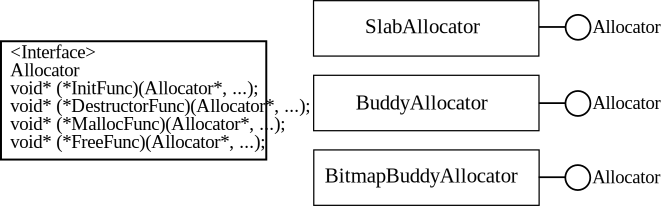
\includegraphics[width=0.8\textwidth]{images/allocator_interface_uml.pdf}
    \caption{Diagramma UML dell'interfaccia Allocator e delle sue implementazioni.}
    \label{fig:uml_allocator_interface}
\end{figure}

Le funzioni di cui manteniamo un riferimento all'interno delle \textit{struct} sono progettate per uso interno: infatti, gli argomenti sono passati attraverso modalità definite dalla libreria di sistema \texttt{<stdarg.h>}. In questo modo, possiamo mantenere i puntatori alle funzioni nonostante per le varie implementazioni della classe essi abbiamo \textit{signature} diverse, dando grande libertà e flessibilità. Contemporaneamente però questa pratica costituisce un rischio, poiché le verifiche sulla correttezza del tipo e del numero degli argomenti non sono fatte a \textit{compile-time}.

Per ovviare a questo problema e permettere al nostro programma di verificare correttamente che i parametri passati siano validi, introduciamo un buffer tra le funzioni interne e l’utente nella forma di funzioni helper segnalate come \textit{inline}. Attraverso esse, il programma mantiene la sua flessibilità internamente senza dover sacrificare in sicurezza: la correttezza dei parametri passati alla chiamata è effettuata dal compilatore e contemporaneamente la performance non è eccessivamente impattata da questo passaggio intermedio grazie alla keyword \textit{inline}. Essa indica al compilatore di ottimizzare aggressivamente la funzione, sostituendo alla chiamata il suo corpo (per questo motivo, è importante che queste funzioni helper siano brevi e concise, in modo da evitare \textit{code bloat}).

Una nota sulla keyword \textit{inline}: è importante ricordare che essa è un suggerimento e non un obbligo, per il compilatore: esistono modalità per forzare questa ottimizzazione, imponendo di applicarla a tutte le chiamate, ma questo potrebbe portare nel lungo termine a una minore ottimizzazione per via della quantità di codice, che renderebbe necessari più \textit{cache swaps} del necessario. Ulteriori test potrebbero mostrarne l’impatto e con ciò l’importanza di lasciare che sia il compilatore a occuparsi delle ottimizzazioni, ma ciò esula dagli scopi dell’analisi.

Ogni classe che implementa l’interfaccia \texttt{Allocator} deve implementare le proprie funzioni interne, che mantengono la stessa signature, e le funzioni \textit{wrapper}, che invece possono avere una signature diversa in base alle necessità. Per esempio, nell’allocazione di memoria per uno SlabAllocator (che velocemente anticipiamo poter allocare unicamente blocchi di memoria di grandezza omogenea) non sarà necessario specificare la grandezza dell’area richiesta. In più, deve fornire anche una rappresentazione grafica del suo stato ai fini di \textit{debugging} e analisi.

Le funzioni helper seguono una nomenclatura più vicina a quella della \textit{libc}, in modo da rendere l’API più intuitiva e immediata. Esse sono:
\begin{itemize}
    \item \texttt{[AllocatorClass]\_create} (wrapper di \texttt{[AllocatorClass]\_init})
    \item \texttt{[AllocatorClass]\_destroy} (wrapper di \texttt{[AllocatorClass]\_dest})
    \item \texttt{[AllocatorClass]\_malloc} (wrapper di \texttt{[AllocatorClass]\_reserve})
    \item \texttt{[AllocatorClass]\_free} (wrapper di \texttt{[AllocatorClass]\_release})
\end{itemize}
Il linker del linguaggio C non permette l'esistenza di funzioni non dichiarate come \textit{static} con nome uguale, ma argomenti diversi (\textit{polimorfismo}). Siamo dunque costretti ad anteporre la classe alla funzione per distinguerle, come vediamo sopra. Sono state esplorate soluzioni a questo problema, ma sfortunatamente introducevano livelli di complessità oppure sacrificavano a livello di \textit{type checking}, come ad esempio avviene con l'utilizzo di \textit{macro}, soluzione comunemente adottata. Grazie alla duplice struttura con funzioni helper e internal sarebbe possibile immagazzinare la specifica classe dell'istanza all'inizializzazione e in base ad essa adoperare la corretta funzione: tuttavia, ciò avrebbe comportato numerose complicazioni nella semplicità e facilità di interpretazione da parte dell'utente.

\subsection{Richiesta iniziale di memoria}
Tutte le classi che implementano l’interfaccia \texttt{Allocator} usano \textit{mmap} per chiedere memoria al sistema operativo. Durante la fase di progetto, è stato valutato alternativamente di poter utilizzare la primitiva \textit{sbrk}, fornita dalla libreria C standard, che permette di “accrescere” l’\textit{heap} esplicitamente. Questo approccio avrebbe permesso un più granulare controllo sulla memoria al costo di una minore flessibilità e, dal punto di vista didattico, avrebbe costituito un'importante opportunità per studiare come avveniva l’allocazione di memoria in versioni precedenti della \textit{sbrk}.
Si è ritenuto tuttavia di usare \textit{mmap} per evitare complicazioni nella deallocazione (la memoria allocata attraverso \textit{sbrk} può infatti essere deallocata solamente in modo sequenziale o si rischia di introdurre frammentazione). La struttura a cui si può accedere attraverso \textit{sbrk} è infatti di tipo LIFO, ossia una pila di memoria. Ciò avrebbe potuto creare problemi laddove gestori fossero distrutti in ordine diverso da quello di creazione o si fosse deciso di permettere l’utilizzo \textit{multithreaded} \footnote{Al netto di possibili complicazioni impreviste, il supporto per l'utilizzo da parte di più entità potrebbe essere aggiunto con relativa facilità adoperando \textit{mutex} per contingentare le operazioni di richiesta e rilascio di memoria.}.

La flag \texttt{MAP\_ANONYMOUS} (anche nota come \texttt{MAP\_ANON}) è stata adoperata alla chiamata di \textit{mmap}. Essa fa sì che la memoria richiesta non sia “supportata” da alcun file. Dal manuale, “The mapping is not backed by any file; its contents are initialized to zero. The fd argument is ignored; however, some implementations require fd to be \texttt{-1}. If \texttt{MAP\_ANONYMOUS} (or \texttt{MAP\_ANON}) is specified, and portable applications ensure this. The offset argument should be zero. for \texttt{MAP\_ANONYMOUS} in conjunction with \texttt{MAP\_SHARED} added in Linux 2.4.” La memoria si trova dunque nella RAM fisica e non fa riferimento a un file \footnote{Chiaramente a meno che non sia stata posta in un file di swap}.

\begin{center}
\begin{tabular}{|l|l|l|}
\hline
Feature & \textit{sbrk} & \textit{mmap}(MAP\_ANONYMOUS) \\
\hline
Memory Type & Heap-only & Any virtual address \\
Fragmentation & High (contiguous heap) & Low (independent mappings) \\
Deallocation & Only last block & Arbitrary (\textit{munmap}) \\
File Backing & No & No (unless explicitly mapped) \\
Modern Usage & Legacy (brk in \textit{malloc}) & Preferred for large allocations \\
\hline
\end{tabular}
\end{center}

% TODO add section about massif and valgrind

\section{La classe SlabAllocator}
Lo \textit{slab allocator} è un gestore pensato per richieste di memoria di taglia costante. La sua struttura interna lo rende adatto quando sono necessarie unicamente allocazioni di memoria di dimensione nota e fissa (ad esempio, un'istanza di una classe): il termine \textit{slab} fa riferimento a questa “fetta” di memoria. Esso è dunque particolarmente efficiente al costo di flessibilità ridotta.

\begin{lstlisting}
struct SlabAllocator {
    Allocator base;
    char* memory_start;
    unsigned int memory_size;
    size_t slab_size;   
    size_t user_size;
    DoubleLinkedList* free_list;   
    unsigned int free_list_size;
    unsigned int num_slabs;
};
\end{lstlisting}

La prima menzione di un’implementazione di \textit{slab allocator} viene descritta nell’articolo di Jeff Bonwick \textit{“The Slab Allocator: An Object-Caching Kernel Memory Allocator”}~\cite{slab} del 1994. In esso vengono elencati i benefici di una soluzione che, rispetto a quella da noi implementata, risulta ben più complessa e strutturata. Il codice di Bonwick infatti trae beneficio non solo dalla taglia definita dei \textit{chunk}, ma anche dalla conoscenza della struttura dei dati che verrà allocata nella memoria richiesta (dichiarata alla creazione del gestore). I blocchi liberi vengono già inizializzati come oggetti e mantengono la loro struttura alla restituzione del blocco, evitando così di dover spendere risorse per riorganizzare la memoria alla prossima richiesta. L’idea consiste nel “preservare la porzione invariante dello stato iniziale di un oggetto nell’intervallo tra gli usi, in modo che essa non debba essere distrutta e ricreata ogni volta che l’oggetto è usato.”

Non scendiamo ulteriormente nei dettagli del gestore di Bonwick per semplicità, ma notiamo che per quanto possa sembrare a posteriori non significativa, l’eleganza della sua soluzione è degna di nota. L’autore dell’articolo infatti non solo definisce algoritmi efficienti e con strumenti approfonditi per il \textit{debugging}, ma si cura di approfondire la relazione tra il suo algoritmo e le strutture del sistema operativo, in particolare con il \textit{Translation Lookaside Buffer}, fornendo chiare evidenze dell’attenzione posta non solo nell’approccio teorico, ma anche all’applicazione pratica del suo gestore. La specializzazione della soluzione applicata da Bonwick la rende ideale per l’utilizzo all’interno di sistemi operativi, che gestiscono spesso numerosi oggetti rappresentati da strutture dati di grandezza nota e fissa (\textit{socket}, \textit{semafori}, \textit{file}…). La prima implementazione di questo modello è presentata nel kernel di SunOS 5.4, per poi comparire a uso interno a molti altri kernel, compreso quello di FreeBSD (v5.0) e Linux (a partire dalla versione 2.1.23), dove successivamente diventerà anche disponibile per l’uso da parte dell’utente.

Nella nostra implementazione non viene fatto \textit{caching} della struttura interna dell’oggetto e l’utente è lasciato libero di gestire liberamente lo slab assegnato. Chiaramente, questo lo rende ordini di grandezza più lento della soluzione applicata da Bonwick. Lo scopo didattico nonostante questo è la dimostrazione di come l’efficienza dei gestori dinamici di memoria sia strettamente correlata alla comprensione da parte del programmatore delle richieste fatte durante il corso della vita dell’applicazione: lo \textit{slab allocator} può essere usato al massimo delle sue potenzialità solo a seguito della profonda comprensione del succedersi delle allocazioni e rilasci di memoria.

\subsection*{Funzionamento dello SlabAllocator}
Come stabilito precedentemente, l’utente non usa le funzioni interne per accedere alle funzionalità del gestore, ma bensì adopera i metodi helper sotto delineati, la cui funzione è puramente quella di "filtro" a tempo di compilazione dei parametri e di gestire in maniera appropriata il valore di ritorno delle funzioni interne

\begin{lstlisting}
inline SlabAllocator* SlabAllocator_create(SlabAllocator* a, size_t slab_size, size_t n_slabs);
inline int SlabAllocator_destroy(SlabAllocator* a);
inline void* SlabAllocator_malloc(SlabAllocator* a);
inline int SlabAllocator_free(SlabAllocator* a, void* ptr);
\end{lstlisting}

L’inizializzazione di un’istanza di SlabAllocator richiede la grandezza dello slab (nei termini di Bonwick, la grandezza dell’oggetto da immagazzinare) e il numero delle stesse. Dopo una serie di controlli sui parametri, la memoria richiesta viene suddivisa in blocchi. Essi sono dunque organizzati in una \textit{linked list}, che mantiene un pratico riferimento alla memoria disponibile e la cui lunghezza massima è pari al numero totale di blocchi. Al termine dell’uso le operazioni di distruzione sono immediate: l’unica accortezza è restituire la memoria al sistema operativo con \textit{unmap}.

\begin{figure}[H]
    \centering
    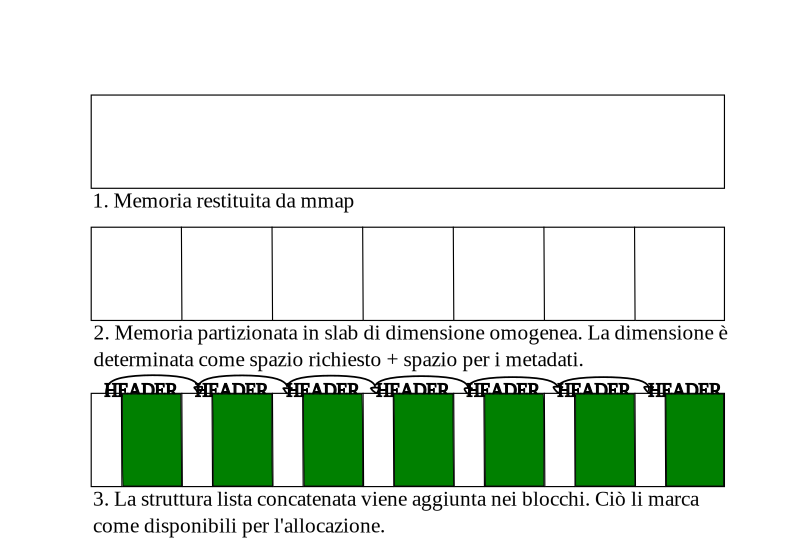
\includegraphics[width=0.8\textwidth]{images/slab/slab_allocator_init.pdf}
    \caption{Inizializzazione dello SlabAllocator: suddivisione della memoria in blocchi di dimensione fissa e organizzazione in una lista concatenata.}
    \label{fig:slab_allocator_init}
\end{figure}

Lo spazio per gestire l’appartenenza del blocco alla lista (ossia i campi di SlabNode, sottoclasse di Node) sono inseriti in cima al blocco. Ciò rende la struttura manipolabile da parte dell’utente, che può inavvertitamente o con intenzioni maligne corromperli scrivendo sopra di essi. A questa problematica sarebbe possibile porre rimedio mantenendo in memoria una struttura dati che tenga un riferimento di tutti gli indirizzi allocati e li possa dunque verificare. Tuttavia, ciò introdurrebbe complicazioni e la scelta implementativa di “fidarsi dell’utente” ricalca quella che è stata adottata nella libc con \textit{malloc}.

Poiché tutti i blocchi hanno la stessa dimensione, alla richiesta non è necessario stabilire quale di essi sia più opportuno allocare: la suddivisione avviene a priori durante l’inizializzazione del gestore, e la taglia dei blocchi non è modificata in nessun momento. La lista viene consultata e il blocco in testa viene estratto e restituito. Quando un blocco viene rilasciato, l’indirizzo di memoria viene controllato: se esso risulta essere corretto, viene semplicemente inserito al primo posto della lista per uso futuro. Notiamo che l’ordine della lista non rappresenta assolutamente la contiguità dei blocchi e richieste immediatamente successive possono ritornare blocchi non contigui.

\subsection*{Efficienza dello SlabAllocator}
Analizziamo più nel dettaglio la complessità computazionale delle operazioni svolte dal gestore. L’allocazione ha un costo costante, così come la liberazione di un blocco, poiché in entrambi i casi viene semplicemente manipolata la testa di una \textit{linked list} contenente i riferimenti ai blocchi liberi. Essi non sono in alcun modo manipolati a seguito di richieste: la loro grandezza rimane costante e questo elimina completamente i costi legati alle operazioni di divisione e unione.

La struttura dello \textit{slab allocator} garantisce che, se è presente almeno uno slab di memoria disponibile, la richiesta dell’utente potrà essere soddisfatta. Tutti i blocchi hanno la stessa dimensione, che viene scelta dal programmatore in fase di inizializzazione, in base alle esigenze specifiche dell’applicazione (ad esempio, la grandezza di una istanza di un oggetto che vi deve essere immagazzinato).

\begin{center}
\begin{tabular}{|l|p{8cm}|}
\hline
Operazione & SlabAllocator \\
\hline
Allocazione & $O(1)$ \\
Deallocazione & $O(1)$ \\
Ricerca blocco libero & $O(1)$ \\
Gestione dello spazio & Dipende dalla scelta iniziale della dimensione dei blocchi \\
\hline
\end{tabular}
\end{center}

L’efficienza dello \textit{slab allocator} è quindi strettamente legata alla scelta iniziale della dimensione dei blocchi. Tuttavia, in scenari dove le esigenze variano nel tempo (ossia si rende necessaria l’allocazione di oggetti di taglia diversa), è possibile combinare più gestori slab, ciascuno ottimizzato per una diversa dimensione. Questo approccio "ibrido" mantiene i vantaggi della complessità costante per le operazioni base, introducendo un trade-off legato alla gestione di più liste separate. La discrepanza tra la dimensione richiesta e quella dello slab più adatto può essere controllata dal programmatore, che può scegliere la configurazione più efficiente per il proprio caso d’uso.

Lo \textit{slab allocator} risulta dunque particolarmente efficace e parsimonioso. Tuttavia, possono verificarsi situazioni in cui slab liberi e inutilizzati occupino memoria inutilmente, ad esempio quando il numero di \textit{chunk} supera quello degli oggetti effettivamente allocati. Le esigenze del programma possono infatti variare nel tempo: talvolta il numero massimo di oggetti che esistono concorrentemente può variare drasticamente. Per ridurre l’occupazione di memoria in questi casi, alcune implementazioni prevedono meccanismi di rilascio (\textit{reclaiming}) degli slab inutilizzati: dopo un periodo di inattività o sotto pressione per memoria, una parte degli slab può essere restituita al sistema operativo. Questa operazione, che comporta un costo aggiuntivo (tipicamente $O(n)$ rispetto al numero di slab da gestire), offre però maggiore flessibilità nell’adattare l’uso della memoria alle necessità correnti. Nel nostro caso, tale funzionalità non è stata implementata.

Rispetto ad altri gestori più generici (come il \textit{buddy system}, esplorati successivamente, o le implementazioni tradizionali di \textit{malloc}), lo \textit{slab allocator} eccelle in rapidità delle operazioni e prevedibilità nell’uso della memoria, risultando particolarmente adatto a sistemi con risorse dedicate e pattern di allocazione ben definiti. La quantità di memoria utilizzata dipende dal numero di slab preallocati, rendendo questa soluzione ideale quando le richieste sono omogenee e pianificabili.

\section{La classe astratta VariableBlockAllocator}
Il problema dell’allocazione di memoria per richieste di dimensioni variabili rimane un tema aperto e ampiamente discusso. Diversi approcci alla sua soluzione sono stati discussi nel tempo, suscitando dibattiti e proposte contrastanti. Sono state sviluppate numerose alternative, ciascuna con i propri vantaggi e limiti, ottenendo livelli di adozione e consenso variabili nell'ambito dei sistemi moderni.

I primi tentativi alla divisione dinamica dello spazio disponibile presero il nome di \textit{“sequential fits”}. In base alle necessità e richieste del programma in esecuzione, la memoria viene divisa in blocchi di dimensione variabile. Essi, organizzati in un'unica lista concatenata, sono esplorati con costo lineare per trovare il \textit{first} (il primo blocco sufficientemente grande) o \textit{best fit} (il blocco più piccolo in grado di soddisfare la richiesta). Se la dimensione del blocco selezionato è maggiore della quantità di memoria necessaria, esso viene partizionato e la memoria in eccesso diventa a sua volta un blocco disponibile. 

Adoperare queste o altre politiche di scelta del blocco tuttavia può comportare la possibilità concreta che, alla richiesta dell'utente, per via della suddivisione in atto dovuta alle allocazioni precedenti, non vi siano blocchi di memoria \textbf{contigua} disponibili per soddisfarla, anche se la quantità di memoria frammentata (o \textit{sparse}) potrebbe esaudire la richiesta. Questa problematica prende il nome di \textbf{frammentazione esterna}.

\begin{lstlisting}
struct VariableBlockAllocator {
    Allocator base;
    size_t internal_fragmentation;
    size_t sparse_free_memory;
};
\end{lstlisting}

La classe astratta \textit{VariableBlockAllocator} implementa l'interfaccia \textit{Allocator}, a cui aggiunge anche campi per monitorare la frammentazione esterna (\lstinline|size_t sparse_free_memory|) e interna (\lstinline[]|size_t internal_fragmentation|), il cui significato sarà esplicitato nella sezione successiva. Quando viene allocata memoria, viene aggiornata la quantità di byte liberi gestiti dall'allocatore in blocchi separati. Se una richiesta non può essere soddisfatta dall'allocatore, vengono controllati questi valori per stabilire se la frammentazione abbia causato il fallimento.

L'implementazione dei \textit{“sequential fits”}, famosamente esplorata da Knuth, presenta importanti limitazioni. La perdità di scalabilità per via del costo lineare è un punto critico: all’aumentare del numero di blocchi, il costo temporale della ricerca diventa proibitivo. Sebbene con dovuti accorgimenti si possano evitare un eccessivo \textit{overhead}\footnote{Knuth stesso ne ha proposto uno che successivamente è diventato molto popolare: il concetto di \textit{boundary tag}, ossia salvare le informazioni al termine dell'area allocata per facilitare la riunione dei blocchi.} e una debilitante frammentazione esterna, l’inefficienza della scansione lineare è il fattore che principalmente ne impedisce l'applicazione nei contesti ad alte prestazioni.

L’evoluzione di questo algoritmo mantiene la divisione dinamica in taglie non prestabilite, ma prova a risolvere il problema della lunghezza eccessiva della lista: investire nell’organizzazione maggiore spazio, gestendo i blocchi liberi più efficientemente, permette di velocizzare la ricerca del blocco corretto. La memoria disponibile viene suddivisa sempre in blocchi liberi, che sono però raccolti in base alla loro taglia in liste diversificate. La struttura è semplice e simile a quella del metodo visto precedentemente, tuttavia grazie alla lunghezza minore delle singolari liste, esse sono più rapidamente esplorabili.

Al momento della richiesta, è esaminata la lista contenente i blocchi della taglia più appropriata, e laddove non vi sia un blocco adeguato vengono ricorsivamente controllate le liste di livello "superiore", contenente blocchi di dimensione maggiore. Il blocco eventualmente individuato è suddiviso e la memoria in eccesso è organizzata in un nuovo \textit{chunk} libero, riposto nella lista corretta secondo la sua grandezza. Questo meccanismo viene chiamato nell’articolo di Wilson et al. \textit{“segregated free lists”}.


\section{La classe BuddyAllocator}
Il \textit{Buddy Allocator} è descritto nella stessa pubblicazione come un “caso particolare” di quest'ultima tipologia di allocatori. Inventato da Harry Markowitz nel 1963 e pubblicato per la prima volta nell’articolo \textit{“A Fast Storage Allocator”}~\cite{knowlton1965} del 1965 da Kenneth C. Knowlton, ingegnere presso Bell Telephone Laboratories, il \textit{buddy system} è facile da implementare e presenta buoni risultati se usato in risposta a richieste di taglia variabile, ma generalmente nota, che vengono ripetute numerose volte.
 
La differenza rispetto agli algoritmi che lo precedono consiste principalmente nelle politiche di \textit{splitting} e \textit{coalescing}. Mentre le metodologie viste finora non stabiliscono esplicitamente regole che l'allocatore debba seguire nel dividere i blocchi liberi per soddisfare le richieste, i \textit{buddy systems} invece stabiliscono una chiara gerarchia che rende il procedimento più ordinato. I blocchi infatti, come approfondiremo successivamente, sono partizionati sempre in metà uguali e riuniti solo quando entrambe le metà sono contemporaneamente libere.

Questa differenza consente di evitare un problema significativo che emerge quando la dimensione dei blocchi non è vincolata. In particolare, modelli di allocazione tipici, come l'alternanza di richieste e rilasci di blocchi di dimensioni diverse, causano frammentazione esterna negli allocatori che adottano metodi come i \textit{sequential fits}. La libertà nella gestione delle dimensioni dei blocchi unita alla ricerca lineare porta alla formazione di numerose aree libere sparse. Gli allocatori con \textit{segregated free lists}, sebbene più efficienti grazie alla suddivisione in liste separate per intervalli di dimensione, non sono immuni al problema. l \textit{Buddy Allocator} rappresentano una possibile soluzione, ma non senza introdurre alcuni compromessi.

\subsection*{Funzionamento del BuddyAllocator}
Ogni blocco di memoria è rappresentato da un \textit{BuddyNode}, che contiene metadati come la dimensione, un’indicazione sullo stato e puntatori al \textit{buddy} e al \textit{parent}. Le informazioni su di essi potrebbero essere raggiunte, note la taglia del blocco e l’indirizzo di partenza, senza bisogno di immagazzinarle esplicitamente nell’header: tuttavia, la scelta di memorizzare queste relazioni, anziché calcolarle dinamicamente attraverso manipolazione degli indirizzi di memoria, semplifica il debug e la visualizzazione dello stato dell'allocatore.

\begin{lstlisting}
typedef struct BuddyNode {
    Node node;
    char *data;
    size_t size; // Size of this block (including header)
    size_t requested_size; // Requested size (for logging)
    int level; // Level in the buddy system
    int is_free; // Whether this block is free
    struct BuddyNode* buddy; // Pointer to buddy block
    struct BuddyNode* parent; // Pointer to parent block
} BuddyNode;
\end{lstlisting}

I nodi sono salvati in una serie di free lists, corrispondenti ai vari livelli di un albero binario. La metodologia è ripresa dalle tecniche elencate precedentemente negli algoritmi \textit{“segregated free lists”}. Alla creazione, viene richiesto all’utente la grandezza dell’area di memoria da gestire e il numero massimo di livelli (alternativamente, poteva essere richiesta la grandezza del blocco di dimensione minima). L'allocatore utilizza due \textit{SlabAllocator} interni: uno per gestire i \textit{BuddyNode} e l'altro per le liste libere, che vengono tutte inizializzate alla creazione. Questa scelta rappresenta un chiaro luogo dove le caratteristiche dello slab allocator possano essere valorizzate, poiché le dimensioni degli oggetti allocati sono fisse e note a priori.

\begin{lstlisting}
typedef struct BuddyAllocator {
    VariableBlockAllocator base; // Base allocator interface
    void* memory_start; // Start of managed memory
    size_t memory_size; // Total size of managed memory
    size_t min_block_size; // Minimum block size (power of 2)
    int num_levels; // Number of levels in the system
    SlabAllocator list_allocator;
    SlabAllocator node_allocator;
    DoubleLinkedList** free_lists;  // Array of free lists for each level (in mmap)
} BuddyAllocator;
\end{lstlisting}


Quando è necessario partizionare un blocco per soddisfare una richiesta, esso viene diviso in parti uguali e i blocchi ottenuti diventano \textit{buddies}, aventi chiaramente la stessa dimensione. Al rilascio da parte dell’utente, il blocco controlla il suo \textit{buddy} e verifica se esso sia a sua volta libero.
Nell’eventualità che entrambi i \textit{buddies} siano contemporaneamente non riservati dall’utente, essi vengono riunificati nel blocco \textit{parent} da cui derivano. Sia l'operazione di divisione dei blocchi che quella di ricongiungimento sono svolte in modo ricorsivo, esplorando tutti i livelli dell'albero fino a che la richiesta non sia stata esaudita o sia stato accertato che non vi siano blocchi liberi per farlo. 

\begin{lstlisting}
// inline has been omitted for brevity
BuddyAllocator* BuddyAllocator_create(BuddyAllocator* a, size_t memory_size, int num_levels);
int BuddyAllocator_destroy(BuddyAllocator* a);
void* BuddyAllocator_malloc(BuddyAllocator* a, size_t size);
int BuddyAllocator_free(BuddyAllocator* a, void* ptr);
\end{lstlisting}

Dalla descrizione del sistema buddy, notiamo facilmente che la struttura dati delineata corrisponde a un albero binario. Infatti, ogni nodo (blocco di memoria) tranne la radice possiede un singolo genitore e un \textit{buddy}. Esso può inoltre a sua volta essere scomposto quando necessario in due ulteriori nodi liberi. Un vantaggio della struttura binaria è che il \textit{buddy} corrisponde sempre con il blocco adiacente (precedente o successivo).

\subsection*{Efficienza del BuddyAllocator}
L'operazione di allocazione esplora per prima la lista libera del livello più appropriato (\textit{best fit}). Se non trova blocchi disponibili, risale ai livelli superiori, dividendo i blocchi fino a raggiungere la dimensione desiderata. Questo approccio garantisce un costo $O(1)$ nel caso ideale (blocco disponibile nel livello corretto) e $O(L)$ nel caso peggiore, dove L è il numero di livelli. La fusione dei blocchi liberi avviene in tempo $O(L)$, grazie alla verifica ricorsiva dello stato del buddy. 
L'uso di \textit{free lists} separate per ogni livello elimina la necessità di strutture talvolta complesse ad albero, semplificando l'implementazione e riducendo il costo. L'allocatore paga un costo in termini di memoria per i metadati aggiuntivi (puntatori a \textit{buddy} e \textit{parent}), che potrebbe essere evitato con un calcolo dinamico degli indirizzi dei buddy. 

L’architettura del \textit{buddy system} risolve radicalmente il problema della frammentazione esterna tipica degli allocatori tradizionali. La memoria libera viene infatti divisa equamente in base alle necessità reali del programma e costantemente riaggregata in blocchi ordinati e perfettamente allineati. Tuttavia, questa soluzione non è esente da criticità. L'arrotondamento sistematico alla potenza di due superiore comporta inevitabilmente una certa quantità di frammentazione interna, particolarmente evidente quando le richieste di memoria sono solo leggermente superiori a una data potenza di due. La rigidità del sistema lo rende dunque meno adatto a gestire pattern di allocazione estremamente variabili o imprevedibili. La differenza tra la memoria richiesta e quella ottenuta viene registrata nel campo \lstinline|size_t internal_fragmentation|.

Ad esempio, supponiamo di avere blocchi disponibili di dimensione $A$, $B$, $C$ e $D$, dove ogni lettera rappresenta una potenza di due crescente (ad esempio, $A = 8$, $B = 16$, $C = 32$, $D = 64$). Se viene richiesta una quantità di memoria pari a $B+1$, il sistema non potrà allocare un blocco di dimensione $B$, ma dovrà assegnare il blocco successivo più grande, ovvero $C$. In questo modo, una richiesta di poco superiore a $B$ comporta l'allocazione di un blocco di dimensione doppia, lasciando inutilizzata una parte significativa della memoria allocata.

\begin{center}
\begin{tabular}{|l|l|}
\hline
Operazione & BuddyAllocator \\
\hline
Allocazione & $O(1)$ / $O(L)$ \\
Deallocazione & $O(1)$ \\
Ricerca blocco libero & $O(1)$ / $O(L)$ \\
Frammentazione interna & Potenzialmente molto alta \\
Frammentazione esterna & Generalmente bassa \\
\hline
\end{tabular}
\end{center}

\section{La classe BitmapBuddyAllocator}
Nelle implementazioni analizzate finora, la ricerca di un blocco libero avviene tramite l'esplorazione di liste concatenate. Se queste sono correttamente ordinate o suddivise per dimensione, la scansione può essere relativamente efficiente quando il blocco cercato è presente. Tuttavia, un problema intrinseco di questo approccio è la possibile discontiguità spaziale dei blocchi nella lista, che può essere causa di inefficienza nella gestione della cache, causando numerosi \textit{miss}.

Per ovviare a questa limitazione, sono stati introdotti allocatori che utilizzano strutture dati più avanzate per memorizzare le informazioni sui blocchi liberi, migliorando così l’efficienza grazie a un utilizzo della cache più avveduto. Nell’articolo di Wilson prendono il nome di \textit{"indexed fit"}. Tra le strutture usate, alberi binari bilanciati (\textit{self-balancing binary trees}) e \textit{heap} si sono dimostrati particolarmente efficaci; ciononostante, essi richiedono un costo gestionale non trascurabile per mantenere l’equilibrio della struttura.

Un approccio alternativo e più semplice rispetto alle strutture dati complesse è l’utilizzo di \textit{bitmap}: questa struttura dati, nota anche come \textit{bit array} o \textit{bit field}, permette di immagazzinare informazioni in modo denso e compatto.  Nella gestione del \textit{BitmapBuddyAllocator}, è fatto uso di una \textit{bitmap} dove ogni bit rappresenta lo stato, libero o occupato, del corrispondente blocco di memoria. A differenza delle liste concatenate (che richiedono dereferenziamenti di puntatori potenzialmente dispersi in memoria, con conseguenti \textit{cache miss}), le bitmap permettono di verificare lo stato dei blocchi in modo più efficiente, poiché le informazioni risiedono in memoria contigua. Ciò può anche avvalersi delle istruzioni SIMD (Single Instruction, Multiple Data) e funzionalità hardware avanzate fornite dall’architettura; tuttavia la problematica della scansione lineare della \textit{bitmap} ricalca la criticità dei metodi \textit{sequential} e \textit{segregated fit}.

Si rende dunque necessario applicare euristiche che restringono l’area di esplorazione a intervalli predefiniti. In questo contesto, il \textit{buddy system} visto nella sezione precedente riemerge come soluzione particolarmente efficace. Grazie alla sua struttura gerarchica binaria, esso permette infatti di individuare rapidamente i blocchi liberi e le relazioni tra di essi, ottimizzando sia l’allocazione che la deallocazione. In particolare, sfruttando una \textit{bitmap} associativa, è possibile delimitare con precisione la zona di memoria in cui cercare i blocchi disponibili, migliorando ulteriormente l’efficienza.

\subsection*{Funzionamento del BitmapBuddyAllocator}
La memoria necessaria per gestire la bitmap viene inserita all'interno dell'area assegnata all'allocatore dall'operazione di \textit{mmap}.
\begin{lstlisting}
typedef struct {
    VariableBlockAllocator base; 
    char* memory_start; // Managed memory area
    int memory_size; // Size of managed memory
    int num_levels; // Number of levels in the hierarchy
    int min_block_size; // Minimum allocation size
    Bitmap bitmap; // Bitmap tracking block status
} BitmapBuddyAllocator;
\end{lstlisting}

Poiché il \textit{BitmapBuddyAllocator} è una variante del classico \textit{buddy system}, le operazioni che esso svolge sono simili a quelle viste precedentemente: la differenza è nella struttura dati che viene consultata (la \textit{bitmap} piuttosto che le liste concatenate). Quando viene richiesta della memoria, l’allocatore cerca in \lstinline[]|bitmap| un blocco libero della dimensione giusta. Se non lo trova, risale di livello per trovarne uno più grande e lo suddivide nei due \textit{buddy} di dimensione uguale, aggiornando la \textit{bitmap} di conseguenza. Un blocco \textit{parent} che sia scomposto in \textit{buddy} di cui almeno uno è utilizzato è segnato a sua volta come non adoperabile per esaudire richieste, in quanto parte di esso è allocata.

\begin{lstlisting}
// inline has been omitted for brevity
BitmapBuddyAllocator* BitmapBuddyAllocator_create(BitmapBuddyAllocator* a, size_t memory_size, int num_levels);
int BitmapBuddyAllocator_destroy(BitmapBuddyAllocator* a);
void* BitmapBuddyAllocator_malloc(BitmapBuddyAllocator* a, size_t size);
int BitmapBuddyAllocator_free(BitmapBuddyAllocator* a, void* ptr);
\end{lstlisting}

Durante la deallocazione, il bit del blocco viene segnato come libero. Se anche il \textit{buddy} è libero, i due vengono fusi e il blocco originario viene ricostruito, riducendo la frammentazione. In breve, il \textit{BitmapBuddyAllocator} unisce la flessibilità del \textit{buddy system} con la velocità e compattezza delle \textit{bitmap}, risultando ideale per ambienti ad alte prestazioni.

\begin{lstlisting}
static int levelIdx(size_t idx) {
    return (int)floor(log2(idx+1));
}

static int buddyIdx(int idx) {
    if (idx == 0) return -1;
    // formula: even goes to idx - 1, odd goes to idx + 1
    if (idx % 2 == 0) {
        return idx - 1; // even index, buddy is left
    } else {
        return idx + 1; // odd index, buddy is right
    }
}

static int parentIdx(int idx) {
    if(idx == 0 ) return -1;
    return (idx - 1) / 2;
}

static int firstIdx(int level) {
    return (1 << level) - 1; // 2^(level-1)
}
\end{lstlisting}

\subsection*{Efficienza del BitmapBuddyAllocator}
Il \textit{BitmapBuddyAllocator} rappresenta un compromesso ottimale tra efficienza (grazie alle ottimizzazioni \textit{bitwise}), semplicità (nessuna gestione di strutture complesse come \textit{self-balancing trees}) e scalabilità (adatto a sistemi con grandi \textit{memory pool}). Mentre il \textit{BuddyAllocator} tradizionale rimane una scelta valida in contesti semplici, in quanto di più facile implementazione, il \textit{BitmapBuddyAllocator} si dimostra superiore in scenari ad alte prestazioni, dove è critico il ruolo del \textit{caching}. 

Questo metodo consente una ricerca estremamente rapida di blocchi contigui liberi, migliorando significativamente la località spaziale e riducendo i problemi di \textit{caching} tipici delle \textit{linked list}. Tuttavia, poiché la verifica della disponibilità richiede comunque l’ispezione sequenziale dei bit (seppur accelerata da ottimizzazioni hardware), la complessità computazionale rimane $O(n)$ per algoritmi come \textit{first-fit} o \textit{best-fit}. Tuttavia, la \textit{internal fragmentation} rimane un problema irrisolto, rendendo questo allocatore meno adatto per carichi di lavoro con richieste di memoria estremamente variabili.

\begin{center}
\begin{tabular}{|l|l|}
\hline
Operazione & BitmapBuddyAllocator \\
\hline
Allocazione & $O(1)$ / $O(L)$ \\
Deallocazione & $O(1)$ \\
Ricerca blocco libero & $O(1)$ / $O(L)$ \\
Frammentazione interna & Potenzialmente molto alta \\
Frammentazione esterna & Generalmente bassa \\
\hline
\end{tabular}
\end{center}
